\section{Now Forecasting Methodology} %3.5

\subsection{K-Fold Cross-validation}
Cross-validation is a statistical method used to evaluate the training effect of machine learning models. The verification data is taken from the training data, but does not participate in the training, so that the matching degree of the model to the data outside the training set can be relatively objectively evaluated. It divides the original data into K groups (K-Fold), makes a validation set for each subset of data, and uses the remaining K-1 subset of data as the training set, so that K models will be obtained. The K models are evaluated in the validation set respectively, and the final MSE is added and averaged to get the cross-validation error. Cross-validation effectively utilizes limited data, and the evaluation result can be as close as possible to the performance of the model on the test set. The recorded relatively excellent hyperparameters are retrained with the optimal model parameters and used as indicators for model optimization\cite{browne2000cross}. Since K-fold cross-validation is suitable for situations where the total amount of data is small, thus it is very suitable for this project. K=10 for this project, i.e.490 data are equally divided into 10 groups, each group contains 49 data.

\begin{figure}[htbp]
    \center
    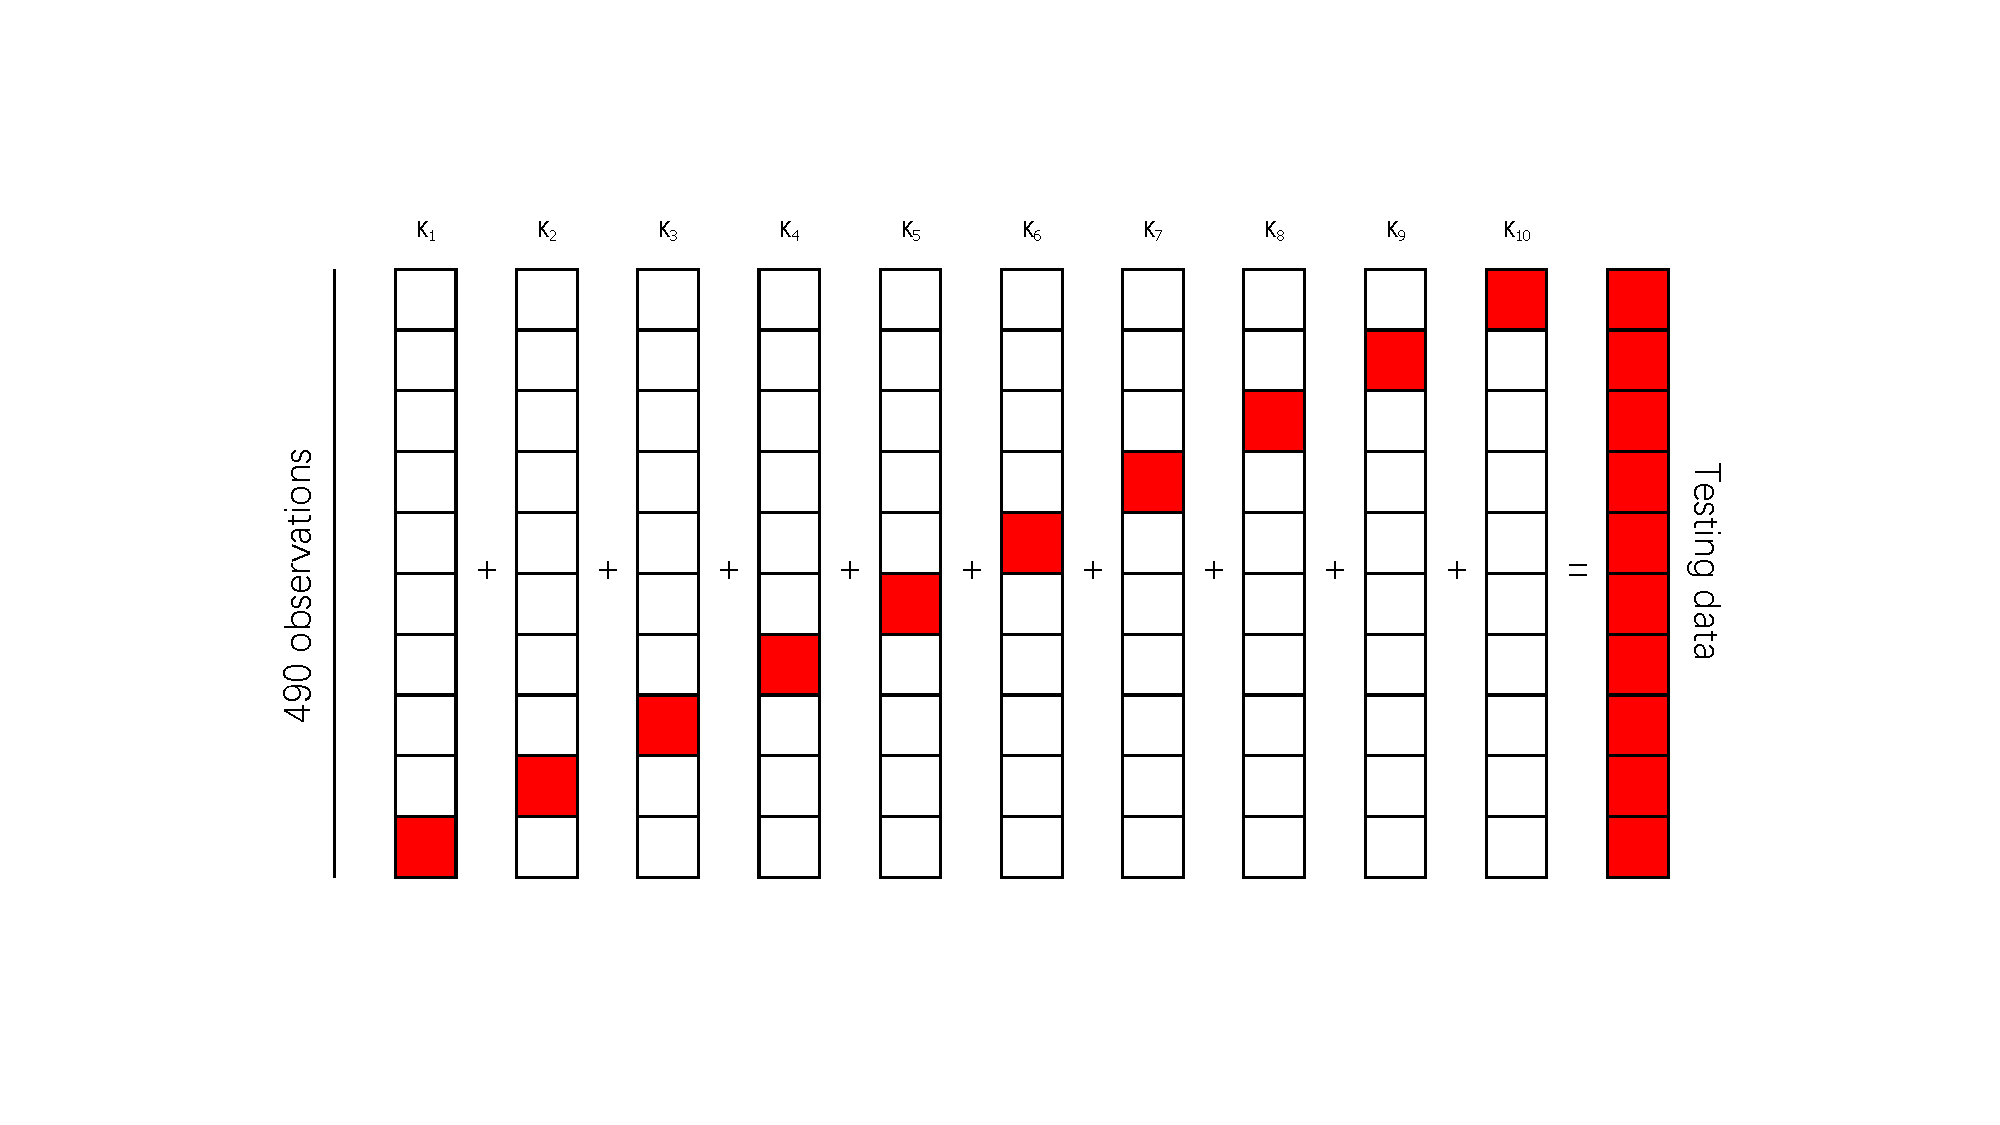
\includegraphics[scale=0.5]{Figure/3.5.1-K-Fold.pdf}
    \caption{K-fold}
\end{figure}


\subsection{Linear Regression}
Linear regression uses statistical analysis to determine the quantitative relationship between multiple variables. Y as the dependent variable and X as the independent variable. To simplify our notation, we also introduce the convention of letting $x_0 = 1$ (this is the intercept term), so that

\begin{eqnarray}
    Y = \sum_{i=1}^{n}{\beta_i x_i}.
\end{eqnarray}


This project uses 7 influencing factors to build a linear regression model. After linear regression calculation, the parameters of each feature in the LR model are obtained. The best-fit straight line is calculated by the least square method, that is, to minimize the sum of squares of the vertical error between each data point and the predicted straight line. P-value can be used to express the magnitude of the significant influence of the independent variable on the dependent variable. In theory, any addition of new variables will increase the R-squared metric\cite{montgomery2012introduction}.

\subsection{Penalised linear regression (Lasso, min/1se)}
Penalty regression is a highly computationally efficient prediction method that can reduce a large number of features into a manageable set and make good predictions on various large data sets, especially when the features are correlated. Penalty regression is a technique to avoid overfitting. Because of the low deviation of linear regression, as the number of features increases, it is susceptible to high variance or overfitting. Add a penalty term as a constraint, that is, the choice of regression coefficient should minimize the sum of the residual square sum and the penalty term to limit the coefficient value and reduce the variance. In penalty regression, the contribution of a feature to the fit of the model must be large enough to offset its penalty. Therefore, only important features that can explain Y can be left\cite{bowles2015machine}.


\begin{eqnarray}
    \sum_{i=1}^{n}{(Y_i-Y_i)^2} + \lambda  \sum_{K=1}^{k}{b_k}
\end{eqnarray}

There are two ways to choose the coefficient $\lambda$ of the penalty term: the minimum (min) method and the 1 standard error (1se) method. The minimum method was selected for this project.



\subsection{Penalised Polynomial Regression (Lasso, min/1se)}
....

\subsection{Random Forest}
Random forest is composed of many decision trees, and there is no correlation between different decision trees. Each decision tree judges and classifies the input samples separately. Each decision tree will get its own classification result. The decision tree with the most classification will become the final the result of. Adjust the parameters on the number of trees and the number of features contained in each tree. The number of trees is determined by out-of-bag error (OOB). When OOB becomes stable, the number at this time is the number of trees\cite{tan2018prediction}. The number of trees selected for this project is 200, with 5 features.

\subsection{Neural Networks}
A neural network is a massively parallel processor composed of simple processing units. Neurons form the basic structure of the network\cite{KO2003271}. When the input enters the neuron, the corresponding weight is assigned, and a nonlinear activation function is applied to convert the input signal into an output signal. This project selected 5 hidden layers, the first hidden layer has 5 neurons, and the second hidden layer has 3 neurons.
